\clearpage
\section{Trigger requirements}
\label{sec:trigger}
% ---- ---- ---- ---- ---- ---- ---- ---- ---- ---- ---- ---- ---- ---- ---- ---- ---- ---- ---- ---- ---- ---- ----

\textbf{We need to find the best way to describe the triggers, here}

%%%%%\subsection{2010 Run A and B}
%%%%%
%%%%%For 2010 run, the analysis exploits single-object-based triggers, developed by the electroweak group 
%%%%%for W and Z boson production studies.
%%%%%
%%%%%Numbers and range obtained by looking at this note \cite{CMS-AN-2010-395}.
%%%%%
%%%%%\subsubsection{Electrons}
%%%%%
%%%%%We select events firing High-Level Trigger (HLT) lines which are seeded on the Level-1 (L1)
%%%%%ECAL trigger. Depending on the running period,
%%%%%we considered photon triggers and then electron triggers. All the triggers
%%%%%used in this analyses were available unprescaled. The specific trigger used for
%%%%%each run period is reported in Table~\ref{tab:2010_EleTrig}.
%%%%%
%%%%%%FIXME Efficiency?
%%%%%%--------------------------------------------------
%%%%%\begin{table}[htbp]
%%%%%\begin{center}
%%%%%{\footnotesize
%%%%%\begin{tabular}{|c|c|c|}
%%%%%\hline
%%%%%Run Range &  HLT Trigger & L1 Trigger                           \\
%%%%%\hline
%%%%%132440-139880  & {\tt HLT\_Photon15\_L1R}                         & {\tt L1\_SingleEG5} \\
%%%%%139965-141882  & {\tt HLT\_Ele15\_LW\_L1R}                        & {\tt L1\_SingleEG5} \\
%%%%%140058-143962  & {\tt HLT\_Ele15\_SW\_L1R}                        & {\tt L1\_SingleEG5} \\
%%%%%141956-144114  & {\tt HLT\_Ele15\_SW\_CaloEleId\_L1R}             & {\tt L1\_SingleEG5} \\
%%%%%146428-147116  & {\tt HLT\_Ele17\_SW\_CaloEleId\_L1R}             & {\tt L1\_SingleEG8} \\
%%%%%147196-148058  & {\tt HLT\_Ele17\_SW\_TightEleIdIsol\_L1R\_v1}    & {\tt L1\_SingleEG8} \\
%%%%%147196-148058  & {\tt HLT\_Ele17\_SW\_TighterEleIdIsol\_L1R\_v1}  & {\tt L1\_SingleEG8} \\
%%%%%148819-149064  & {\tt HLT\_Ele17\_SW\_TighterEleIdIsol\_L1R\_v2}  & {\tt L1\_SingleEG8} \\
%%%%%149181-149442  & {\tt HLT\_Ele17\_SW\_TighterEleIdIsol\_L1R\_v3}  & {\tt L1\_SingleEG8} \\
%%%%%\hline
%%%%%\end{tabular}
%%%%%\caption[.]{\label{tab:2010_EleTrig}
%%%%%Summary of electron triggers.}}
%%%%%\end{center}
%%%%%\end{table}
%%%%%%--------------------------------------------------
%%%%%
%%%%%\subsubsection{Muons}
%%%%%
%%%%%For the muons, all the triggers
%%%%%used in this analyses were available unprescaled. The specific trigger used for
%%%%%each run period is reported in Table~\ref{tab:2010_MuTrig}.
%%%%%
%%%%%%--------------------------------------------------
%%%%%\begin{table}[htbp]
%%%%%\begin{center}
%%%%%{\footnotesize
%%%%%\begin{tabular}{|c|c|c|}
%%%%%\hline
%%%%%Run Range &  HLT Trigger & L1 Trigger                           \\
%%%%%\hline
%%%%%132440-147116  & {\tt HLT\_Mu9}            & {\tt L1\_SingleMu7} \\
%%%%%146428-148058  & {\tt HLT\_Mu11}           & {\tt L1\_SingleMu7} \\
%%%%%147196-149442  & {\tt HLT\_Mu15\_v1}       & {\tt L1\_SingleMu7} \\
%%%%%148819-149182  & {\tt HLT\_IsoMu13\_v3}    & {\tt L1\_SingleMu7} \\
%%%%%149291-149442  & {\tt HLT\_IsoMu13\_v3}    & {\tt L1\_SingleMu7} \\
%%%%%\hline
%%%%%\end{tabular}
%%%%%\caption[.]{\label{tab:2010_MuTrig}
%%%%%Summary of muon triggers.}}
%%%%%\end{center}
%%%%%\end{table}
%%%%%%--------------------------------------------------

\subsection{2011 run}

During the first period of 2011 run, until the 3$^{rd}$ May technical stop, the instantaneous luminosity
was smaller than $1\cdot10^{33}\percms$, which allowed to rely on single-lepton triggers for both
the $e$ and the $\mu$ channels.


\begin{table}[htb]
  \begin{center}
  \begin{tabular}{r|c}
  \hline
  HLT path  - $e$ channel & Run range \\
  \hline
  \scriptsize{\texttt{HLT\_Ele27\_CaloIdVT\_CaloIsoT\_TrkIdT\_TrkIsoT\_v*}} & \scriptsize{160404 - 163869} \\
  \scriptsize{\texttt{HLT\_Ele17\_CaloIdVT\_CaloIsoT\_TrkIdT\_TrkIsoT\_CentralJet30\_CentralJet25\_PFMHT15\_v*}} & \scriptsize{165088 - 165633} \\
  \scriptsize{\texttt{HLT\_Ele25\_CaloIdVT\_CaloIsoT\_TrkIdT\_TrkIsoT\_CentralJet30\_CentralJet25\_PFMHT20\_v*}} & \scriptsize{165970 - 166967} \\
  \scriptsize{\texttt{HLT\_Ele22\_CaloIdVT\_CaloIsoT\_TrkIdT\_TrkIsoT\_CentralJet30\_CentralJet25\_PFMHT20\_v*}} & \scriptsize{167039 - 167913} \\
  \hline
  \end{tabular}
  \end{center}
  \caption{Summary of HLT path used used and run ranges of applicability for the electron channel.}
  \label{tab:HLTelectron}
\end{table}%

\begin{table}[htb]
  \begin{center}
  \begin{tabular}{r|c}
  \hline
  HLT path  - $\mu$ channel & Run range \\
  \hline
  \scriptsize{\texttt{HLT\_IsoMu24\_v*}} & \scriptsize{160404 - 167913} \\
  \hline

  \end{tabular}
  \end{center}
  \caption{Summary of HLT path used used and run ranges of applicability for the muon channel.}
  \label{tab:HLTmuon}
\end{table}%


%%%%%For 2011 run the expected instantaneous luminosity is such that rates of single-object-based triggers will become too high
%%%%%to be substainable. The best example is given by single electron trigger which, already at the beginning of 2011 run,
%%%%%when ${\cal{L}}^{ist} \ = \ 5 \cdot 10^{32} \ cm^{-2}s^{-1}$, will be at an accettable rate ($\sim 15\ Hz$) for an 
%%%%%$E_T$ threshold around $35\ GeV$; such requirement will cause a drop in efficiency, for the same offline cuts applied 
%%%%%on 2010 data, of about $30\%$ (Fig.\ref{fig:SingleEleTrigger}).\\
%%%%%
%%%%%A solution is naturally emerging in VBF analyses, since the complex topology of the studied final states, i.e.
%%%%%one isolated lepton and two eta-separated jets, can be used to reduce the rate without affecting the trigger 
%%%%%efficiency on signal events. 
%%%%%
%%%%%\begin{figure}[htb]
%%%%%  \begin{center}
%%%%%    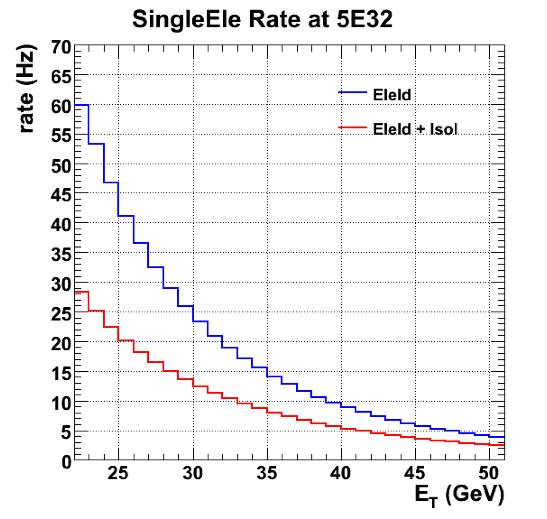
\includegraphics[width=0.45\textwidth]{plots/SingleEleRates_5E32.png}
%%%%%    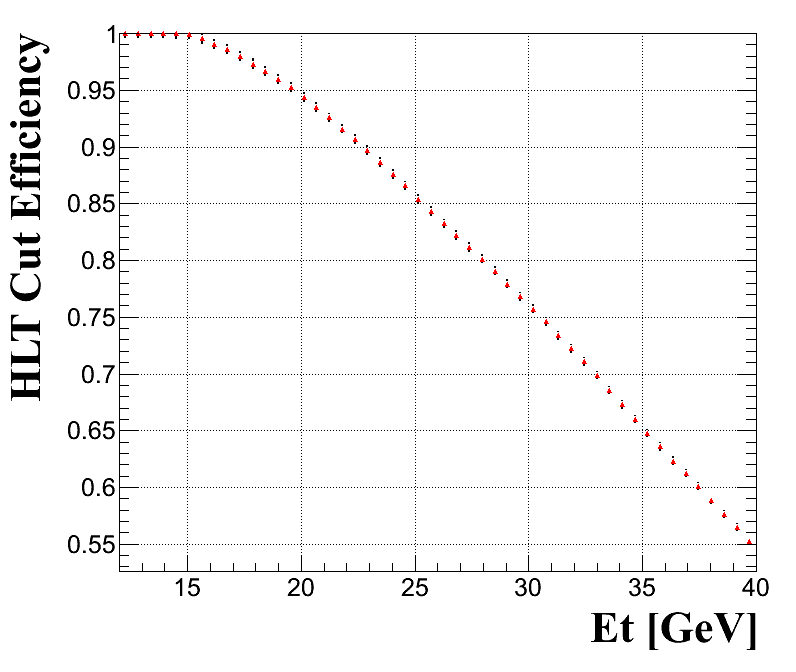
\includegraphics[width=0.45\textwidth]{plots/SingleEleEfficiencies_5E32.png}
%%%%%    \caption{Single electron High-Level-Trigger rate (left) and efficiencies (right). Rate projections are
%%%%%             done for an instantaneous luminostity of  $\ 5 \cdot 10^{32}\ cm^{-2}s^{-1}$ while efficiencies
%%%%%             are evaluated on a $H\rightarrow WW\rightarrow \ell \nu_{\ell} + qq'$ sample.}
%%%%%    \label{fig:SingleEleTrigger}
%%%%%  \end{center}
%%%%%\end{figure}
%%%%%
%%%%%\subsubsection{Electrons}
%%%%%
%%%%%Given the high fake rate, the electron channel is the one that exploits most extensively the multi-object-based triggers
%%%%%(AKA cross-triggers)\footnote{For the L1 seeding we keep relying on pure ECAL trigger, but other possibilities are presented 
%%%%%in appendix \ref{app:L1}}. For this channel we have developed an HLT based on one isolated and identified electron (see Table 
%%%%%\ref{table:EleVbtfCuts}) and two jets separated in $\eta$. The tuning of the cuts on each object is obtained 
%%%%%by choosing the set of cuts which maximizes the signal efficiecy at a given rate, which for us is about $10\ Hz$.
%%%%%To simplify this multi-dimensional optimization problem we have used the offline selection, which 
%%%%%in principle must remain the same of 2010, which requires, in a simplified version:
%%%%%\begin{itemize}
%%%%% \item the presence of at least one electron passing VBTF electron ID WP 80
%%%%% \item the presence of at least a pair of jets (Jet1, Jet2) with
%%%%%  \begin{itemize}
%%%%%    \item [$\cdot$] transverse energies greater than ($40\GeV$, $25\GeV$) 
%%%%%    \item [$\cdot$] a pseudorapidity separation greater than $3.5$ 
%%%%%  \end{itemize}
%%%%%\end{itemize}
%%%%% 
%%%%%Hence we fixed the HLT cut on the hard jet of the pair at $35\GeV$, to avoid a loss in signal events 
%%%%%due to HLT turn on curve in jet reconstruction, and we reproduced the VBTF electron ID WP 80 at trigger level.\\
%%%%%
%%%%%To find the best cuts on the soft jet $E_T$, the electron $E_T$ and the jet $\Delta \eta$ separation we split the study 
%%%%%in two branches:
%%%%%\begin{enumerate}
%%%%% \item Fix the cut on electron and soft jet $E_T$ at $15 \ GeV$ and $20\ GeV$ respectively and examine
%%%%%the rate and efficiency dependance on the $\Delta \eta$ cut (Fig. \ref{fig:EleTrigger_Deta})
%%%%% \item Fix the cut on $\Delta \eta$ at $2$ and examine
%%%%%the rate and efficiency dependance on electron and soft jet $E_T$ (Fig. \ref{fig:EleTrigger_EleEt_JetEt})  
%%%%%\end{enumerate}
%%%%%
%%%%%The study shows that by requiring a cut on the electron $E_T$ of $15 \ GeV$, on the soft jet $E_T$ of $20\GeV$ and
%%%%%on the the jet pair $\Delta \eta$ of $2$ we can obtain an HLT efficiency on signal events of $93 \%$ while using 
%%%%%an HLT bandwidth of $3.9 \ Hz$ at ${\cal{L}}^{ist} \ = \ 5 \cdot 10^{32} \ cm^{-2}s^{-1}$. This working point is 
%%%%%mostly interesting because the prospected lumi for late 2011 run is $10^{33} \ cm^{-2}s^{-1}$,
%%%%%so that we may be able to use the same HLT path for the entire data taking period.
%%%%%
%%%%%\begin{figure}[htb]
%%%%%  \begin{center}
%%%%%    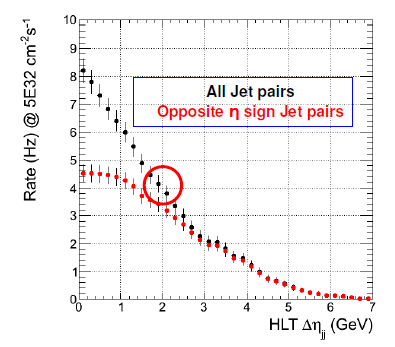
\includegraphics[width=0.45\textwidth]{plots/HLT_dEta_Rate.png}
%%%%%    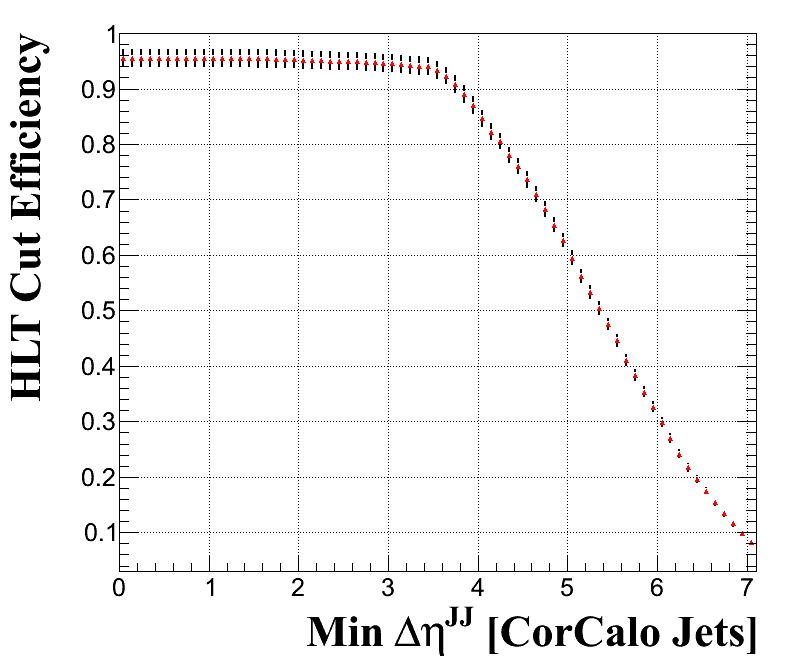
\includegraphics[width=0.45\textwidth]{plots/HLT_dEta_Eff.png}
%%%%%    \caption{Electron plus Di-Jet rate (left) and efficiencies (right). Distributions are obtained with 
%%%%%             the following additional HLT requirements : VBTF WP 80 electron with $E_T\ > \ 15 \ GeV$ and soft
%%%%%             jet $E_T> \ 15 \ GeV$ }
%%%%%    \label{fig:EleTrigger_Deta}
%%%%%  \end{center}
%%%%%\end{figure}
%%%%%
%%%%%\begin{figure}[htb]
%%%%%  \begin{center}
%%%%%    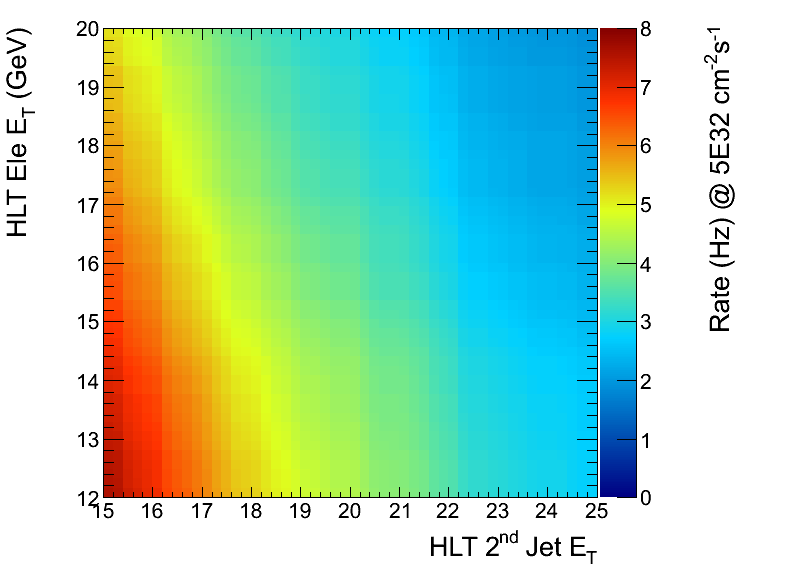
\includegraphics[width=0.45\textwidth]{plots/HLT_EleEt_JetEt_Rate.png}
%%%%%    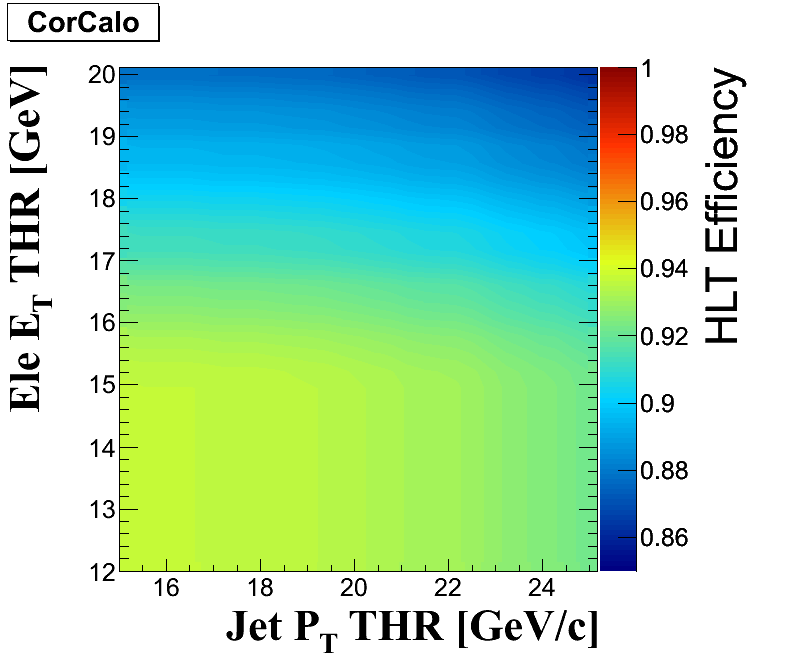
\includegraphics[width=0.45\textwidth]{plots/HLT_EleEt_JetEt_Eff.png}
%%%%%    \caption{Electron plus Di-Jet rate (left) and efficiencies (right). Distributions are obtained with 
%%%%%             the following additional HLT requirements : electron passing VBTF Id WP 80 and
%%%%%             jet $\Delta \eta \ > 2$ }
%%%%%    \label{fig:EleTrigger_EleEt_JetEt}
%%%%%  \end{center}
%%%%%\end{figure}
%%%%%
%%%%%\subsection{turn-on curves}
